\section{Segment retransmisson over HTTP/2}
\label{sec:retrans}

After introducing the basics of segment retransmission for ABR streaming and outlining its drawbacks in the case of HTTP/1.1 in Sect.~\ref{subsec:retrans_sched}, we introduce the usage of this approach in the case of HTTP/2 in this section. We first give an overview on the advantages and disadvantages of using our retransmission approach in the case of HTTP/2 over TCP and QUIC, respectively. This is followed by a description of the implementation of our approach. Results from an evaluation of this approach are presented in Sect.~\ref{sec:eval}.

\subsection{Example}
\label{subsec:example}
In the following, we compare a segment retransmission approach that is based on HTTP/2 over TCP (the current standard) with one that is based on HTTP/2 over QUIC. The TCP-based approach is shown in Fig.~\ref{fig:retr_tcp}. Here, we show a specific scenario of retransmissions for ABR streaming. In this scenario, HTTP/2 over TCP allows the multiplexing of multiple requests within a single TCP connection. This feature makes this approach more efficient than our existing HTTP/1.1 solution, since original  segment transmissions and retransmission can be performed in parallel. (In the case of HTTP/1.1, segments can either only be transmitted sequentially or a new TCP connection has to be established for the retransmissions). Despite the support of multiplexing several requests over a single TCP connection, this approach has several drawbacks. First of all, HOL blocking can lead to stalling. Such a case is indicated in Fig.~\ref{fig:retr_tcp}, where the first retransmitted TCP segment is lost. All of the following (original and retransmitted) TCP segments will be blocked from delivery to the application layer until the lost TCP segment is successfully received. This HOL blocking, caused by a TCP segment retransmission, prevents original segments from being delivered to the buffer of the video player. 
This can result in an incorrect estimate of the segment download rate and consequently an unnecessary reduction in bit rate quality for the download of future original segments. In the worst case, this causes the drainage of the video player buffer, which in turn will stall the video playout.

In contrast, an HTTP/2 over QUIC approach is not impacted by HOL blocking. Fig.~\ref{fig:retr_quic}, shows the same segment transmission scenario as in Fig.~\ref{fig:retr_tcp}. As opposed to the scenario shown in Fig.~\ref{fig:retr_tcp}, the QUIC-based approach does not prevent the original datagrams from being delivered to the video player buffer if the first retransmitted UDP datagram is lost. This should lead to a significant reduction in the risk of stalling and misinterpretation of the download rate. In addition, the application can decide if the lost retransmitted UDP datagram should be retrieved again or not. 
This decision can be based on buffer fill level, position of the retransmitted segment in the buffer, and observed download rate. With the use of QUIC, the application can also determine at which rate segments should be downloaded. For example, pacing~\cite{quic_pacing} can be applied for the retransmission of segments to assure that such transmissions only minimally interfere with the transmission of original segments.

\begin{figure*}[htb]
  \centering     
  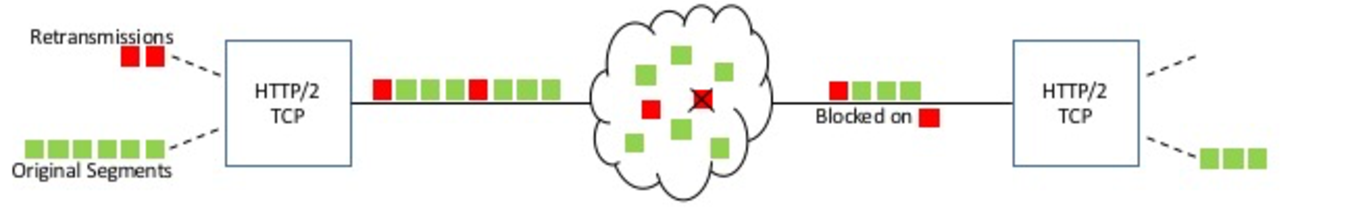
\includegraphics[width=.9\textwidth]{figures/retr_tcp.pdf}
  \centering
  \caption{This figure shows a scenario of original and retransmitted segment transmission in the case of HTTP/2 over TCP. The first of the retransmitted TCP segments (red) is lost, which leads to HOL blocking at the receiver.}
  \label{fig:retr_tcp}
  \vspace{-15pt}
\end {figure*}

\begin{figure*}[htb]
  \centering
  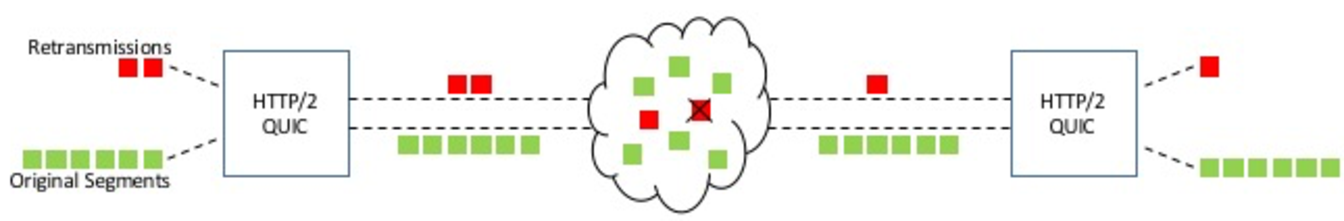
\includegraphics[width=.9\textwidth]{figures/retr_quic.pdf}
  \caption{This figure shows a scenario of original and retransmitted segment transmission in the case of HTTP/2 over QUIC. In contrast to Fig.~\ref{fig:retr_tcp}, the loss of a retransmitted UDP datagram (red) does not lead to HOL blocking and all original segments are delivered to the video player buffer.}
  \label{fig:retr_quic}
\end {figure*}

\subsection{Implementation}
\label{subsec:impl}
In this section, we give an overview of our implementation of ABR streaming that is based on HTTP/2 over QUIC that enables retransmissions of segments that have originally been transmitted in a low(er) quality (see Sect.~\ref{subsec:retrans_sched}).

\subsubsection{SQUAD with HTTP/2 and HTTP/1.1}
Since the multiplexing feature of HTTP/2 is unavailable in its predecessor, HTTP/1.1, the original version of SQUAD implements retransmission scheduling as a series of GET requests where at any given time there is only one outstanding request to the ABR streaming server. Intuitively, such a sequential implementation stalls the application pipeline and can lead to either conservative retransmission scheduling or a severe buffer drain.
To prevent stalling in case of a severe drop in measured download rate, SQUAD implements retransmission abandonment, which cancels segment retransmission when we observe that the segment will not be downloaded on time.
Our HTTP/2 implementation converts this sequential behavior into a parallel, multiplexed session of two simultaneous GET requests, where, at any given time there are a maximum of two possible streams active within a single connection. SQUAD is implemented as part of an open-source Python-based DASH player emulator, \texttt{AStream}.\footnote{\url{https://github.com/pari685/AStream}} For ease of integration, we use the Python-based HTTP/2 library, \texttt{hyper}\footnote{\url{https://github.com/Lukasa/hyper}}, in order to implement two multiplexed GET requests for original and retransmission segment downloads. Additionally, we implement multithreading to allow transmissions on both HTTP/2 streams to proceed independently. We note that HTTP/2 still uses the same TCP connection which suffers from HOL blocking as explained in Sect.~\ref{subsec:example}. and therefore, we also implement a SQUAD over QUIC approach which is introduced next. In order to make a fair comparison, we also adapt the original implementation of SQUAD to use \texttt{hyper} for making HTTP/1.1 requests.

\subsubsection{SQUAD with QUIC}
Similar to the experiment above, we implement multiplexed sessions for original and retransmitted segment downloads using QUIC. However, we include the use of IPC message streams with minimal overhead to communicate between the QUIC client (implemented in C++) and the AStream player (implemented in Python). Unlike HTTP/2 over TCP, QUIC does not suffer from HOL blocking and is designed to deliver data to the application as soon as they arrive at the receiver and a stream within a QUIC connection is not adversely affected by events that cause delay or loss of packets on a parallel, ongoing stream. At the time of this implementation, we used Chromium for Linux with QUIC version \texttt{Q043}. In order to provide support for multiplexed streams for SQUAD, we perform the following modifications on the \texttt{QUIC client}\footnote{\url{https://www.chromium.org/quic/playing-with-quic}} code provided by Google: (i) we create and synchronize simultaneous streams within a single connection, (ii) we introduce IPC messaging not only to send commands between AStream and QUIC but also to provide intermediate chunk download rate measurements to the SQUAD ABR algorithm.

We note that this work does not focus on modifying SQUAD to perform optimally with a protocol such as QUIC but is instead intended as a study to evaluate  the performance of SQUAD retransmissions over QUIC in order to determine if QoE can be improved with such an approach.